\documentclass[10pt]{beamer}

\usetheme{metropolis}
\usepackage{appendixnumberbeamer}

\usepackage{booktabs}
\usepackage[scale=2]{ccicons}

\usepackage{pgfplots}
\usepgfplotslibrary{dateplot}

\usepackage{xspace}

\usepackage{tikz}
	\usetikzlibrary{shapes.geometric, arrows, positioning}
	\tikzstyle{startstop} = [rectangle, rounded corners, minimum width=3cm, minimum 		height=1cm,text centered, draw=black, fill=red!30]
	\tikzstyle{io} = [trapezium, trapezium left angle=70, trapezium right angle=110, minimum width=3cm, minimum height=1cm, text centered, draw=black, fill=blue!30]
	\tikzstyle{process} = [rectangle, minimum width=3cm, minimum height=1cm, text centered, draw=black, fill=orange!30]
\tikzstyle{decision} = [diamond, minimum width=3cm, minimum height=1cm, text centered, draw=black, fill=green!30]
\tikzstyle{arrow} = [thick,->,>=stealth]
\tikzstyle{arrow} = [thick,->,>=stealth]
%\usepackage{listings}
\usepackage{minted}

\usepackage{bm}%................................. Bold math symbols (after fonts)

\setbeamercolor{normal text}{bg=white}





\title{EML4930/EML6934: Lecture 11}
\subtitle{Scikit-Learn: Machine learning and \textbf{Regression}}
\date{November 9, 2017}
%\author{CJ}
\author{Charles Jekel}
%\titlegraphic{\includegraphics{images/avatarCropped.png}\vspace{58cm}}
%\institute{1. University of Florida\\ 2. Stellenbosch University, South Africa}

% \titlegraphic{\hfill\includegraphics[height=1.5cm]{logo.pdf}}

\begin{document}

\maketitle


\begin{frame}[fragile]{Quiz feedback}
\begin{minted}
{python}
# let's consider an arbitrary function
def my_fun():
    return
    
# this won't execute the function, nor will it pass an error
my_fun

# infact I can even create an alias name of the function
new = my_fun

# again this won't execute the function
new

# You need to use () to execute a function
new()
\end{minted}
\end{frame}

\begin{frame}[fragile]{Quiz feedback plotting}
\begin{minted}
{python}
import numpy as np
import matplotlib.pyplot as plt

x = np.linspace(0,20)
y = 2.0*x - .3

plt.figure()
plt.plot(x,y)
plt.show # this doesn't display the figure, 
# it's just the name of the function!

# you need to execute the function in order 
# to display the figure
plt.show()
\end{minted}
\end{frame}

\begin{frame}{Topic for today: Scikit-Learn}
\begin{itemize}
\item    Simple and efficient tools for data mining and data analysis
\item    Accessible to everybody, and reusable in various contexts
\item    Built on NumPy, SciPy, and matplotlib
\item    Open source, commercially usable - BSD license
\end{itemize}

Dr. Jake VanderPlas’s Python Data Science
Handbook: Essential Tools for Working with Data. \url{http://shop.oreilly.com/product/0636920034919.do}

The textbook available for free in the form of Jupyter notebooks which
can be viewed at \url{https://github.com/jakevdp/PythonDataScienceHandbook}  or \url{http://nbviewer.jupyter.org/github/jakevdp/PythonDataScienceHandbook/blob/master/notebooks/Index.ipynb}
\end{frame}

\begin{frame}{Scikit-Learn has great documentation}
with plenty of tutorials and examples for each class... You should take a look at it

\url{http://scikit-learn.org/}

\end{frame}

\begin{frame}{What is classification? - Supervised learning}
\begin{itemize}
\item Given a collection of labeled features: Can we find a pattern in the features to predict the labels?
\item Classification is used everywhere!
\item Ex: You are applying for a loan. The bank knows your income, job stability, and debt. Are you approved for the load?
\item Features: income, job stability, debt
\item Labels: approve or reject
\item Binary classification problem!
\end{itemize}
\end{frame}

\begin{frame}{New iPhone X - unlock with your face}
\begin{figure}

\includegraphics[width=1.0\textwidth]{figs/iphonex.png}
\end{figure}
\end{frame}

\begin{frame}{Classification example 1}
\begin{figure}
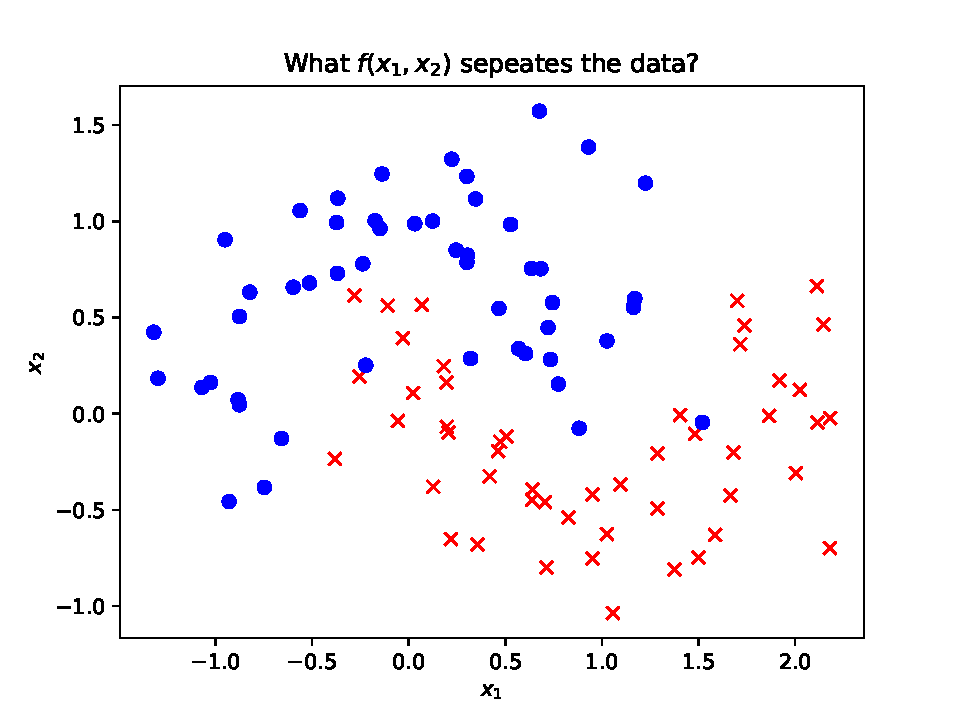
\includegraphics[width=1.0\textwidth]{figs/1.pdf}
\end{figure}
\end{frame}

\begin{frame}{Classification example 2}
\begin{figure}
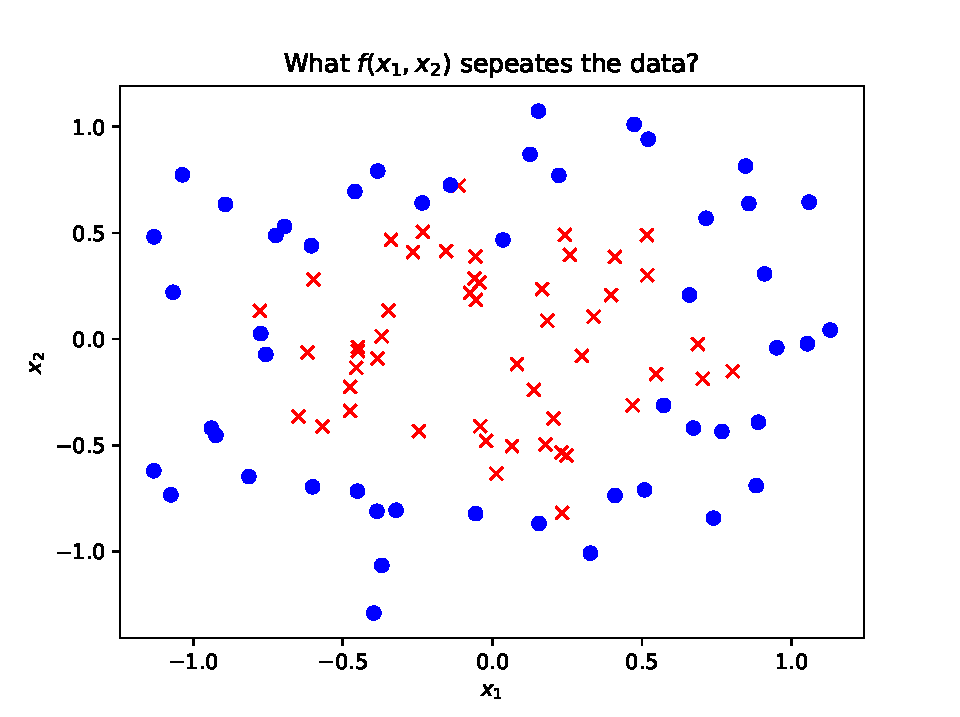
\includegraphics[width=1.0\textwidth]{figs/2.pdf}
\end{figure}
\end{frame}

\begin{frame}{Classification example 3}
\begin{figure}
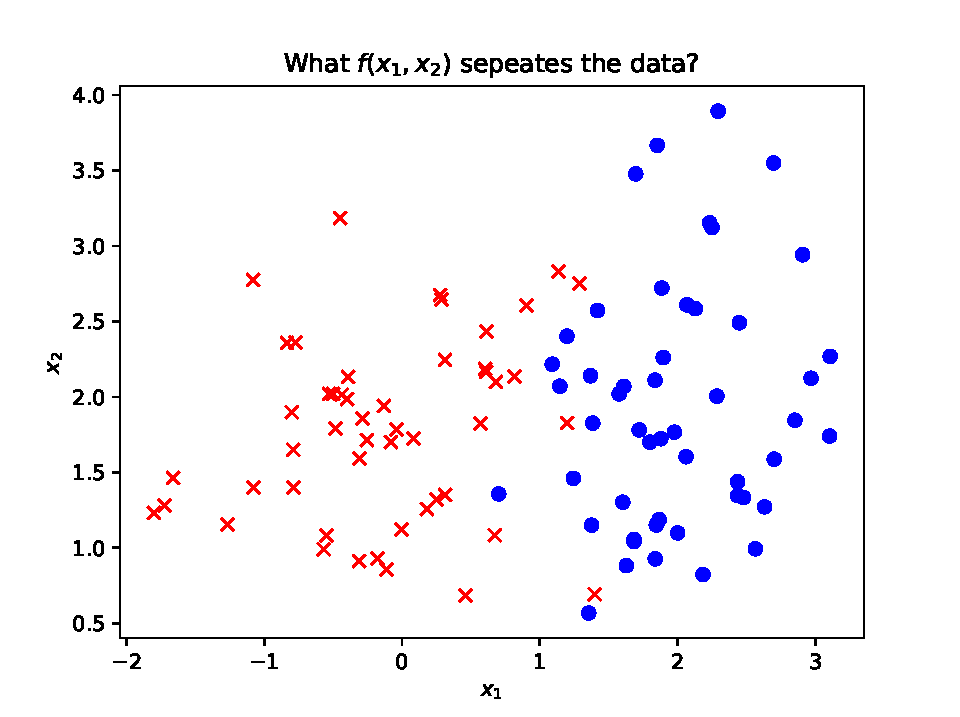
\includegraphics[width=1.0\textwidth]{figs/3.pdf}
\end{figure}
\end{frame}

\begin{frame}{What is regression? }
\begin{itemize}
\item Can we find the trend in data?
\item Can we predict the values in-between data points? 
\item Classification is used everywhere!
\item Ex: You are applying for a loan. The bank knows your income, job stability, and debt. How much of a loan can you get approved for?
\item Variables: income, job stability, debt
\item Output: How much \$ you get?
\end{itemize}
\end{frame}

\begin{frame}{Linear regression: fitting a line to data}
\begin{figure}
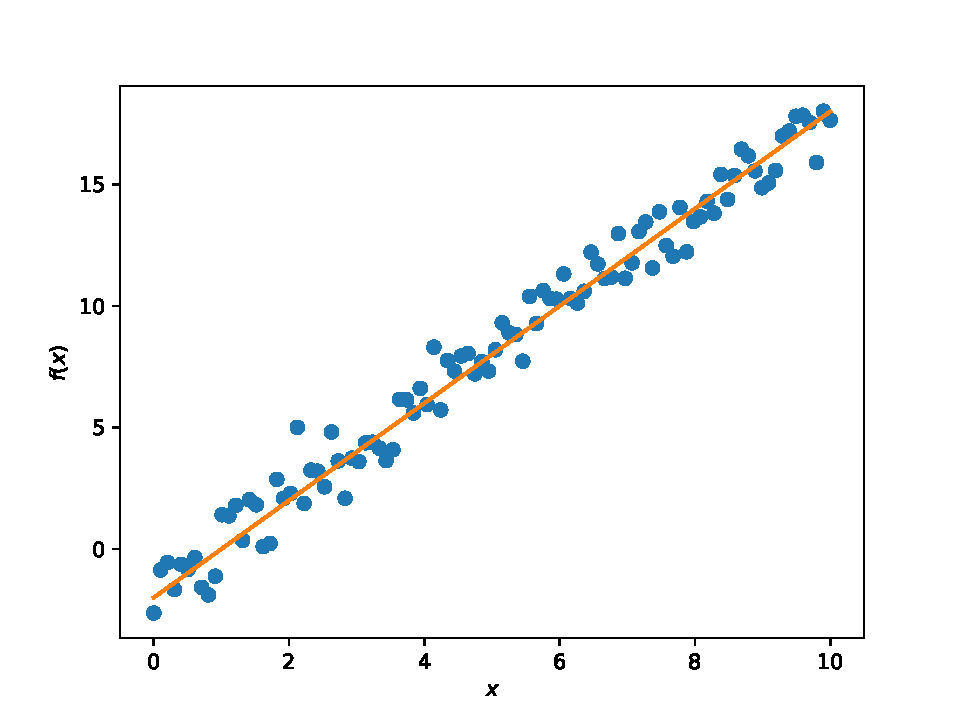
\includegraphics[width=1.0\textwidth]{figs/linear_regression.pdf}
\end{figure}
\end{frame}

\begin{frame}{Kriging: using correlation between data}
\begin{figure}
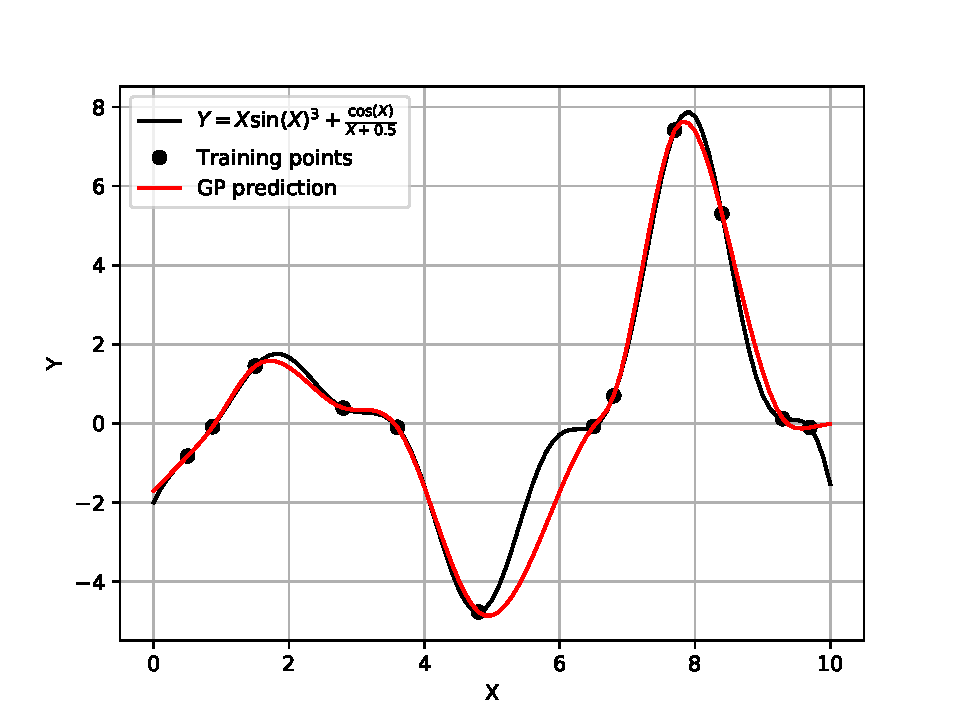
\includegraphics[width=1.0\textwidth]{figs/Kriging.pdf}
\end{figure}
\end{frame}

\begin{frame}{What is clustering? Unsupervised learning}
\begin{itemize}
\item Can we find the structure in data?
\item Can we detect and identify groups in data?
\item Ex: We have a bunch of data related to income, job stability, and debt. Can we identify a pattern in the data?
\item The key is that we don't know the label or value. 
\item Ex: Used to identify similarities in protein chains 
\end{itemize}
\end{frame}

\begin{frame}{Clustering: Can we categorize this data?}
\begin{figure}
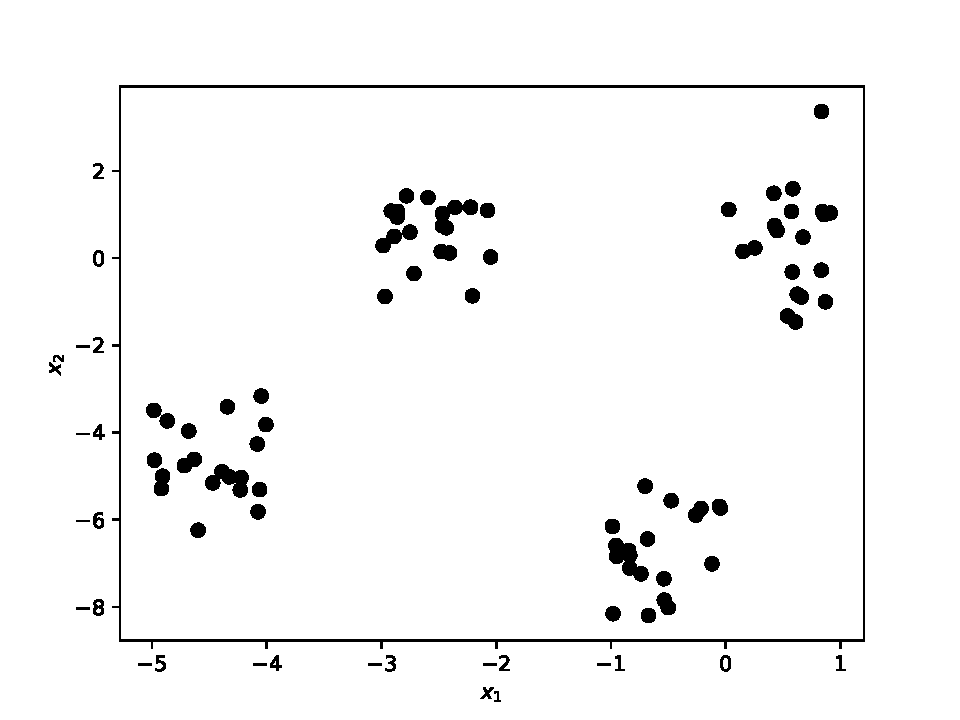
\includegraphics[width=1.0\textwidth]{figs/clust.pdf}
\end{figure}
\end{frame}

\begin{frame}{Clustering output}
\begin{figure}
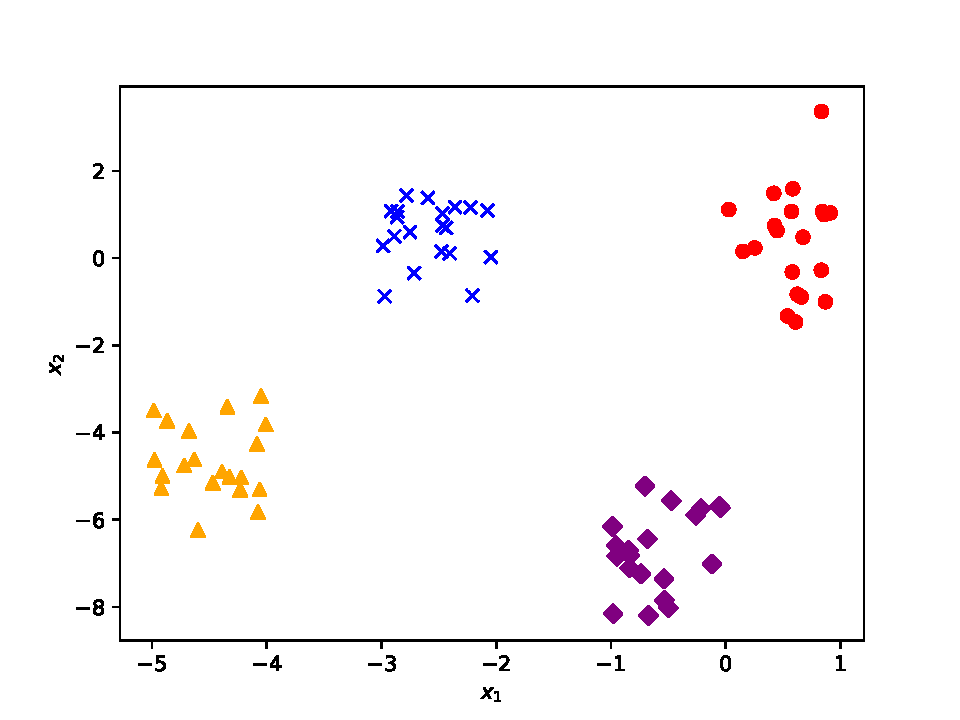
\includegraphics[width=1.0\textwidth]{figs/cluster.pdf}
\end{figure}
\end{frame}

\begin{frame}{So what does the data look like for Scikit-Learn}
Out input data will be a matrix (or numpy array) with $n$ number of samples and $d$ number of design variables (or \textbf{features})
\begin{equation}
\bm{X} = \begin{bmatrix}
x_{11} & x_{12} & x_{13} & \cdots & x_{1d} \\ 
x_{21} & x_{22} & x_{23} & \cdots & x_{2d} \\ 
x_{31} & x_{32} & x_{33} & \cdots & x_{3d} \\ 
\vdots & \vdots * \vdots & \vdots & \vdots \\
x_{n1} & x_{n2} & x_{n3} & \cdots & x_{nd} \\ 
\end{bmatrix}
\end{equation}
Each row of $\bm{X}$ represents a single sample.


Out output data will be a vector $\bm{y}$ (usually a numpy array) with $n$ number samples.
\begin{equation}
\bm{y} = \begin{bmatrix}
y_{1} \\
y_{2} \\
y_{3} \\
\vdots \\
y_{n} \\
\end{bmatrix}
\end{equation}
\end{frame}

\begin{frame}[fragile]{Let's consider a simple linear regression example}
\begin{minted}
{python}
import numpy as np
import matplotlib.pyplot as plt

# let's create some arbitrary data
# and fit a line to it

np.random.seed(33)
x = 10.0*np.random.random(100)
noise = np.random.normal(loc=0.5, size=100)
y = 2.3*x - 3 + noise
plt.figure()
plt.plot(X,y, 'o')
plt.show()
\end{minted}
\end{frame}

\begin{frame}[fragile]{Building a linear regression model}
\begin{minted}
{python}
from sklearn.linear_model import LinearRegression
# LinearRegression is a Python class that we'll use to create
# our linear model object

# we can't pass a vector into scikit-learn
# instead we need to pass a feature matrix
# we can do this by reshaping x
X = x.reshape(-1,1)

# we initialize a model object from the LinearRegression class
# to begin the process. With the initialization, we can pass
# model hyper-parameters, in this case we pass that a 
# y intercept be determined
model = LinearRegression(fit_intercept=True)
\end{minted}
\end{frame}

\begin{frame}[fragile]{Fitting the linear regression model}
\begin{minted}
{python}
# simply pass your training data into the model's fit function
# which will run an 'optimization' selecting the best parameters
# == this is the same as an ordinary least squares fit ==
model.fit(X,y)

# in this case there are two parameters for the line 
# y = mx + b
print('m = ', model.coef_)
print('b = ', model.intercept_)
# score calculates the R^2 (Coefficient of determination) 
# for a given input and output 
my_score = model.score(X,y)

print('R^2 = ', my_score)
\end{minted}
\end{frame}

\begin{frame}[fragile]{Predicting for new $x$ values}
\begin{minted}
{python}
# let's generate new x values from slightly smaller than min(x)
# to the slightly larger than the max(x)
x_hat = np.linspace(np.min(x)-1.0,  np.max(x)+1.0, 100)

# Again x_hat is a vector, and must be reshaped 
# to be a 2 dimensional array
X_hat = x_hat.reshape(-1, 1)

# we can find new y_hat values by using the model.predict function
y_hat = model.predict(X_hat)

# let's plot the results
plt.figure()
plt.plot(X,y, 'o')
plt.plot(x_hat, y_hat, '-')
plt.show()
\end{minted}
\end{frame}

\begin{frame}[fragile]{What about polynomials?}
So let's consider a toy polynomial problem where
\begin{equation}
y = \beta_0 + \beta_1 x + \beta_2 x^2
\end{equation}
on the domain $-10.0 \leq x \leq 10.0$

\begin{minted}
{python}
# generate artificial data
np.random.seed(19)
x = (10.0 + 10.0)* np.random.random(100) - 10.0
noise = np.random.normal(scale=5.0,size=100)
y = -1.0 + 2.2*x - 0.5*x**2 + noise

plt.figure()
plt.plot(x,y, 'o')
plt.show()
\end{minted}
\end{frame}

\begin{frame}[fragile]{Scikit-Learn includes a polynomial prepossessing tool}
So in order the least squares regression, we need to construct the regression matrix $\bm{X}$. Scikit-Learn includes a Polynomial class for doing this easily.
\begin{minted}
{python}
from sklearn.preprocessing import PolynomialFeatures
# again we need to transfer x to a matrix... 
# the reason is that sklearn doesn't deal with 1D data...
X = x.reshape(-1,1)

# create a poly object from the PolynomialFeatures class
# in our case we'll be fitting a second order polynomial
poly = PolynomialFeatures(degree=2)

# now we use poly to transform our X into a Regression matrix!
X = poly.fit_transform(X)
print(X)
# note this transformation includes the y intercept!
\end{minted}
\end{frame}

\begin{frame}[fragile]{Fitting the second order polynomial}
\begin{minted}
{python}
# create quad object from linear regression
# the default is that fit_intercept = False
# we don't want fit_intercept because it's included in X
quad = LinearRegression(fit_intercept=False)

# perform the least squares fit
quad.fit(X,y)

# predict for new values of x
x_hat = np.linspace(np.min(x), np.max(x), 100)
x_hat = x_hat.reshape(-1,1)
X_hat = poly.fit_transform(x_hat)
y_hat = quad.predict(X_hat)

# plot the results
plt.figure()
plt.plot(x,y, 'o')
plt.plot(x_hat, y_hat, '-')
plt.show()
\end{minted}
\end{frame}

\begin{frame}[fragile]{What are the resulting parameters?}
Recall \begin{equation}
y = \beta_0 + \beta_1 x + \beta_2 x^2
\end{equation}

You $\beta$ parameters are stored in the quad object.
\begin{minted}
{python}
print('beta0 =', quad.coef_[0])
print('beta1 =', quad.coef_[1])
print('beta2 =', quad.coef_[2])
\end{minted}
\end{frame}

\begin{frame}[fragile]{What about polynomials for higher dimensions?}
Consider a polynomial response surface\begin{equation}
f(x_1,x_2) = \beta_0 + \beta_1 x_1 + \beta_2x_2 + \beta_3x_1^2 + \beta_4x_1x_2 + \beta_5x_2^2
\end{equation}
\begin{minted}
{python}
# let's generate a 2 dimensional polynomial problem
np.random.seed(121)
X = np.random.random((100,2))
# since this is a matrix, there is no need to reshape
y = 1.0 + X[:,0] + 0.9*X[:,1] + 1.2*X[:,0]**2  \
-1.3*X[:,0]*X[:,1] - 3.0*X[:,1]**2
# plot the data
from mpl_toolkits.mplot3d import Axes3D
import matplotlib.pyplot as plt
fig = plt.figure()
ax = fig.add_subplot(111, projection='3d')
ax.scatter(X[:,0], X[:,1], y, 'o')
ax.set(xlabel='$x_1$', ylabel='$x_2$', zlabel='$f(x_1,x_2$')
fig.show()
\end{minted}
\end{frame}

\begin{frame}[fragile]{Same process for creating regression matrix and fitting}
\begin{minted}
{python}
from sklearn.preprocessing import PolynomialFeatures
poly = PolynomialFeatures(degree=2)
X_train = poly.fit_transform(X)


# fit the model
model = LinearRegression(fit_intercept=False)
model.fit(X_train,y)
# print the model coefficients - you'll see they are exact!
print(model.coef_)

# Let's generate sampeles to predict over the domain
x = np.linspace(np.min(X), np.max(X), 10)
x1,x2 = np.meshgrid(x,x)
X_hat = np.zeros((100,2))
X_hat[:,0] = x1.flatten()
X_hat[:,1] = x2.flatten()
\end{minted}
\end{frame}

\begin{frame}[fragile]{Predicting and comparing the result}
\begin{minted}
{python}
X_test = poly.fit_transform(X_hat)

# predict for X_test
Y_hat = model.predict(X_test)

# reshape y_hat
y_hat = Y_hat.reshape((10,10))

# plot the results
fig = plt.figure()
ax = fig.add_subplot(111, projection='3d')
ax.plot_surface(x1, x2, y_hat)
ax.scatter(X[:,0], X[:,1], y, 'o', color='black')
ax.set(xlabel='$x_1$', ylabel='$x_2$', zlabel='$f(x_1,x_2$')
fig.show()
\end{minted}
\end{frame}

\begin{frame}[fragile]{Classifcation with the famous flower database...}
Naive Bayes Classification of Iris dataset...
\begin{minted}
{python}
import seaborn as sns
iris = sns.load_dataset('iris')

X_iris = iris.drop('species', axis=1)
y_iris = iris['species']  

# sklearn includes tools for validation and model selection
from sklearn.cross_validation import train_test_split
Xtrain, Xtest, ytrain, ytest = train_test_split(X_iris, y_iris, random_state=1)   
# this code splits the entire dataset into two
# a training set and a testing set
\end{minted}

\end{frame}

\begin{frame}[fragile]{The process for fitting models is same: apply NB}
\begin{minted}
{python}
# 1. choose model class
from sklearn.naive_bayes import GaussianNB 

# 2. instantiate model
model = GaussianNB()  
   
# 3. fit model to data                  
model.fit(Xtrain, ytrain)   

# 4. predict on new data                
y_hat = model.predict(Xtest)

# 5. score the model
print(model.score(Xtest,ytest))          
\end{minted}
\end{frame}


%\begin{frame}{Symbolic math with SymPy}
%SymPy is a Python library for symbolic mathematics. It aims to become a full-featured computer algebra system (CAS) while keeping the code as simple as possible in order to be comprehensible and easily extensible. SymPy is written entirely in Python. 
%
%\url{http://www.sympy.org}
%
%Documentation: \url{http://docs.sympy.org/latest/index.html}
%
%Tutorial: \url{http://docs.sympy.org/latest/tutorial/index.html}
%\end{frame}
%
%\begin{frame}{What's in SymPy}
%Way more than what we can cover in a single lecture
%\begin{itemize}
%\item Arbitrary precision
%\item Integration, integral transforms
%\item Equations, inequalities, Diophantine equations, differential equations, Recurance relations
%\item Number theory
%\item Boolean algebra
%\item Tensors 
%\item Probability 
%\item Group theory
%\end{itemize}
%\end{frame}
%
%\begin{frame}{What's missing from SymPy}
%\begin{itemize}
%\item Graph theory 
%\item Quantifier elimination
%\item Control theory
%\item Coding theory
%\end{itemize}
%For a full comparison of every computer algebra system visit this wiki \url{https://en.wikipedia.org/wiki/List_of_computer_algebra_systems}
%\end{frame}
%
%\begin{frame}{SymPy is a Python library}
%\begin{itemize}
%\item SymPy is a pure Python library 
%\item If you can't do it in Python, then you can't do it in SymPy
%\item SymPy does not change, modify, or add to the Python language
%\item SymPy will be easy and intuitive if you know Python
%\end{itemize}
%\end{frame}
%
%\begin{frame}[fragile]{Symbolic expression one variable at a time}
%\begin{minted}
%{python}
%from sympy import *
%
%# create symbolic variables x, y, z
%x = Symbol('x')
%y = Symbol('y')
%z = Symbol('z')
%\end{minted}
%
%It's recommended to assign the variable name to the symbol of the same. 
%\end{frame}
%
%\begin{frame}[fragile]{You can assign multiply symbolic variables at once}
%\begin{minted}
%{python}
%
%# create symbolic variables w, x, y, z
%w, x, y, z = symbols('w x y z')
%\end{minted}
%There are a few things to note:
%\begin{itemize}
%\item use \mint{python}|Symbol()| to create a single symbolic variable
%\item use \mint{python}|symbols()| to create multiple symbolic variables where each variable is separated by a space
%\item all items are case-sensitive
%\item Symbol() is different from symbol()
%\end{itemize}
%\end{frame}
%
%\begin{frame}[fragile]{Symbolic expressions}
%\begin{minted}
%{python}
%a = 3.0*x**2 - 2.0*x + 1.0
%
%# we can do math on symbolic expressions
%a = a*x +1
%
%# simplify a
%a = a.simplify()
%# equivalent to a = simplify(a)
%\end{minted}
%\end{frame}
%
%
%
%\begin{frame}[fragile]{Symbolic equalities}
%\begin{minted}
%{python}
%# Eq is an equality object
%# this is how to express x+1 = 4 in SymPy
%b = Eq(x+1,4)
%\end{minted}
%\end{frame}
%
%\begin{frame}[fragile]{Are two symbolic representations equal?}
%It's impossible to show that two symbolic expressions are equal in general 
%\url{https://en.wikipedia.org/wiki/Richardson%27s_theorem}
%\begin{minted}
%{python}
%a = cos(x)**2 - sin(x)**2
%b = cos(2*x)
%
%# to see if a == b we could do
%print(simplify(a-b))
%
%# or we can use equals()
%print(a.equals(b))
%
%# these methods are not perfect!
%\end{minted}
%\end{frame}
%
%\begin{frame}[fragile]{Rationals in SymPy}
%\begin{minted}
%{python}
%# let's express 1/3 as a rational
%a = Rational(1,3)
%b = Integer(1)/Integer(3)
%\end{minted}
%\end{frame}
%
%\begin{frame}[fragile]{Substitution}
%\begin{minted}
%{python}
%a = x*y**2 + y*x**2
%
%# to evaluate at x = 1, y = 2, use dictionary
%a.subs({x:1, y:2})
%
%# to substitute y = x^2
%a.subs(y, x**2)
%
%# note that a is immutable! .subs() does not change a!
%
%\end{minted}
%\end{frame}
%
%\begin{frame}{Printing symbolic math in SymPy}
%There are several printers available in SymPy
%\begin{itemize}
%\item str
%\item stepr
%\item ASCII pretty printer
%\item Uncode pretty printer
%\item \LaTeX
%\item MathML
%\item Dot
%\end{itemize}
%\end{frame}
%
%\begin{frame}[fragile]{initialize printing}
%\begin{minted}
%{python}
%init_printing()
%# that's it to start the pretty printing process
%\end{minted}
%If you are in a qtconsole
%\begin{itemize}
%\item and have \LaTeX installed, the printer will use \LaTeX to create images of the expressions
%\item and don't have \LaTeX installed, the printer will use Matplotlib's MathJax to render \LaTeX
%\end{itemize}
%If you are in a normal Python session
%\begin{itemize}
%\item unicode printer
%\item ASCII printer
%\end{itemize}
%
%\end{frame}
%
%
%\begin{frame}[fragile]{Printing options and pprint}
%You can set \LaTeX and unicode to false if you just want to use ASCII printing
%\mint{python}| init_printing(use_latex=False, use_unicode=False) |
%
%on my Windows System (in a normal command prompt) the unicode detector isn't working...
%
%Additionally there is a unicode pretty printer
%\mint{python}|pprint( x**2+3) |
%
%If you'd rather use ASCII then you'll have to specify
%\mint{python}|pprint(x**2+3, use_unicode=False) |
%\end{frame}
%
%\begin{frame}[fragile]{Getting the \LaTeX from an expression is easy}
%\begin{minted}
%{python}
%a = latex(x**2*y + x*y**2)
%# a is a latex string
%print(a)
%\end{minted}
%\end{frame}
%
%\begin{frame}[fragile]{Simplification functions}
%\begin{table}
%\begin{tabular}{ll}
%\textbf{Function} & \textbf{Description}  \\
%\hline
%simplify()  & Attempt to intelligently Express the simplest function  \\
%expand()  & Expanding polynomial expressions \\
%factor()  & Factors a polynomial into irreducible factors over rationals \\
%collect() & Collects common powers of a term in an expression \\
%cancel() & Take a rational and put into standard form (no common factors) \\
%apart() & Partial fraction decomposition \\
%trigsimp() & Simplify expression using trigonometric identities \\
%expand\_trig() & i.e. apply sum or double angle identities \\
%\end{tabular}
%\end{table}
%\end{frame}
%
%\begin{frame}[fragile]{Exponential and log}
%\begin{minted}
%{python}
%a = ln(x)
%# same as a = log(x)
%
%b = exp(x)
%
%# if needed you can specify that x, y are strictly positive with
%x, y = symbols('x y', positive=True)
%
%# alternatively you can specify that n is a real number
%n = symbols('n', real=True)
%\end{minted}
%\end{frame}
%
%\begin{frame}[fragile]{Special functions}
%\begin{minted}
%{python}
%x, y, z = symbols('x y z')
%k, m, n = symbols('k m n')
%
%# factorial
%factorial(x)
%
%# binomial coefficient 
%binom(n, k)
%
%# gamma function
%gamma(z)
%
%# generalized hypergoemetric function 
%hyper([1,2], [3], z)
%\end{minted}
%\end{frame}
%
%\begin{frame}{Let's just take a moment to appreciate Python and SymPy}
%There is a lot that SymPy has to offer, more so that I can go over today. If you want to learn everything. Work through the (very long Tutorial -- it may take you a few hours...) \url{http://docs.sympy.org/latest/tutorial/} 
%
%Remainder of what I'm going to cover:
%\begin{itemize}
%\item Calculus (derivatives, integrals, limits)
%\item Solvers 
%\item Matrix operations
%\end{itemize}
%\end{frame}
%
%\begin{frame}[fragile]{derivatives}
%\begin{minted}
%{python}
%# to take derivatives use the diff function
%
%y = x**3 + 2.0*x**2 - 4.0*x - 10.0
%
%# take the derivative with respect to x (dy/dx)
%diff(y,x)
%
%# take the second derivative with respect to x  (d**2y/dx**2)
%diff(y,x,x)
%
%# take the third derivative with respect to x (d**3y/dx**3)
%diff(y,x,x,x)
%
%\end{minted}
%\end{frame}
%
%\begin{frame}[fragile]{derivatives - object oriented approach...}
%\begin{minted}
%{python}
%# to take derivatives use the diff function
%
%y = x**3 + 2.0*x**2 - 4.0*x - 10.0
%
%# take the derivative with respect to x (dy/dx)
%y.diff(x)
%
%# take the second derivative with respect to x  (d**2y/dx**2)
%y.diff(x,x)
%
%# take the third derivative with respect to x (d**3y/dx**3)
%y.diff(x,x,x)
%
%# note y is not changed when you do this (y is immutable) 
%\end{minted}
%\end{frame}
%
%\begin{frame}[fragile]{Integrals - indefinite}
%\begin{minted}
%{python}
%y = cos(x)
%
%# take the integral of y with respect to x
%integrate(y,x)
%
%# or 
%y.integrate(x)
%
%# note this does not include constant!!!
%# you must add constants manually!
%\end{minted}
%\end{frame}
%
%\begin{frame}[fragile]{Integrals - definite}
%\begin{minted}
%{python}
%y = 1 /  x**3 
%
%# take the integral of y with respect to x from 1 to infinity (oo) that's o twice
%# (integration_variable, lower_limit, upper_limit)
%integrate(y, (x, 1, oo))
%y.integrate((x, 1, oo))
%
%# these two lines are the same!
%\end{minted}
%\end{frame}
%
%\begin{frame}[fragile]{Limits}
%\begin{minted}
%{python}
%y = 1 /  x**3 
%
%# take the limit of y as x goes to infinity
%limit(y, x, oo)
%
%# take the limit of y as x goes to zero from the positive
%limit(y, x, o, '+')
%
%# take the limit of y as x goes to zero from the negative
%limit(y, x, o, '-')
%\end{minted}
%\end{frame}
%
%\begin{frame}[fragile]{Solve an equation}
%\begin{minted}
%{python}
%y = x**2 - 2.1*x + 4.0
%
%# solve for when y = 0
%solve(y,x)
%
%# solve for when y = 4
%solve(Eq(y,4),x)
%\end{minted}
%There is more! Read \url{http://docs.sympy.org/latest/tutorial/solvers.html}
%\begin{itemize}
%\item linear system solvers
%\item non-linear system solvers
%\item differential equation solvers
%\end{itemize}
%\end{frame}
%
%\begin{frame}[fragile]{Matrices in SymPy}
%\begin{minted}
%{python}
%# NOTE: Matrix are the only mutable SymPy object
%M = Matrix([[1, 3], [-2, 3]])
%N = Matrix([[0, 3], [0, 7]])
%# add two matrices 
%M + N
%# Matrix multiplication
%M*N
%
%# Multiply a matrix
%3*M
%
%# same as M*M
%M**2
%
%# invert a Matrix
%M**-1
%\end{minted}
%\end{frame}
%
%\begin{frame}{Functions for matrix manipulation}
%\begin{table}
%\begin{tabular}{ll}
%\textbf{Function} & \textbf{Description}  \\
%\hline
%rref() & Reduce row echelon form \\
%nullspace() & Find the nullspace of a matrix \\
%eigenvals() & Find the eigenvalues of a matrix \\
%eigtenvects() & Find the eigenvectors of a matrix \\
%det() & Compute the determinant of matrix
%\end{tabular}
%\end{table}
%
%You can use these functions as methods of the Matrix object as well...
%\end{frame}
%
%\begin{frame}{End of SymPy}
%SymPy is very powerful!
%
%Hopefully this will be useful. 
%\end{frame}
%
%\begin{frame}{Design of experiments (DOE) with pyDOE}
%The pyDOE package is designed to help the scientist, engineer, statistician, etc., to construct appropriate experimental designs.
%
%\url{https://pythonhosted.org/pyDOE/}
%
%Capabilities
%\begin{itemize}
%\item General Full-Factorial (fullfact)
%\item 2-Level Full-Factorial (ff2n)
%\item 2-Level Fractional-Factorial (fracfact)
%\item Plackett-Burman (pbdesign)
%\item Box-Behnken (bbdesign)
%\item Central-Composite (ccdesign)
%\item Latin-Hypercube (lhs)
%\end{itemize}
%\end{frame}
%
%\begin{frame}{latin-hypercube random sampling}
%lhs(n, samples=10, criterion='c', iterations=5)
%    
%    \textbf{Parameters}
%    
%    n : int
%        The number of factors to generate samples for
%        (consider this the number of design variables)
%    
%   \textbf{Optional}
%
%    
%    samples : int
%    
%        The number of samples to generate for each factor (Default: n)
%    
%    criterion : str
%    
%        Allowable values are "center" or "c", "maximin" or "m", 
%        "centermaximin" or "cm", and "correlation" or "corr". If no value 
%        given, the design is simply randomized.
%        
%    iterations : int
%    
%        The number of iterations in the maximin and correlations algorithms
%        (Default: 5).
%\end{frame}
%
%
%\begin{frame}[fragile]{lhs use}
%\begin{minted}
%{python}
%from pyDOE import lhs
%import matplotlib.pyplot as plt
%lhd = lhs(2, samples=5, criterion='cm')
%# my design variables are available as
%x_1 = lhd[:,0]
%x_2 = lhd[:,1]
%
%# NOTE: the outuput of your variables will always be [0,1]
%# so you'll need to scale your variables accordingly
%
%# scatter plot of the design over the domain
%plt.figure()
%plt.plot(x_1,x_2, 'o')
%plt.grid(True)
%plt.xlim((0,1))
%plt.ylim((0,1))
%plt.show()
%\end{minted}
%\end{frame}

%

%\begin{frame}{Reminder: Quiz at the end of next class (11/02/2017)}
%\begin{itemize}
%\item Quiz will cover anything from lecture 00 - lecture 05
%\item You should be able to write the code to plot a curve in Python from memory!
%\item Sample quiz questions will be posted
%\item I view lectures 00 - 05 as the basics of Python (these are the lectures the final exam will be about! + this lecture for reading and writing files) Lectures 06 - 13 build upon these basics for advanced cases. 
%\end{itemize}
%\end{frame}
%
%\begin{frame}{Let's take a look at HW 09}
%\begin{itemize}
%\item You are presented with a practical structural optimization problem
%\item You must create a couple functions to aid in the optimization
%\item One function will take read an input template and write a modified version of the file
%\item The other function reads specific values from a large output file
%\item This HW is to prepare you for \textit{black-box} optimization (think of the input template and output file your results from some expensive simulation that you'll be running!)
%\end{itemize}
%\end{frame}
%
%\begin{frame}{Topics for today's lecture}
%\url{https://docs.python.org/3/tutorial/inputoutput.html}
%\begin{itemize}
%\item with statement
%\item open function
%\item methods for file objects
%\item read file line by line
%\item string manipulation
%\item itertools islice efficient loops
%\item read a csv file
%\item write a csv file
%\end{itemize}
%\end{frame}
%
%\begin{frame}{I've created a demo.txt file which contains the following}
%This is line 1 of a demo txt file. 
%
%This is line 2 of a demo txt file. 
%
%This is line 3 of a demo txt file. 
%
%This is line 4 of a demo txt file.
%
%This is line 5 of a demo txt file.
%
%This is line 6 of a demo txt file.
%
%This is line 7 of a demo txt file.
%
%This is line 8 of a demo txt file.
%
%This is line 9 of a demo txt file.
%
%This is line 10 of a demo txt file.
%
%I replace\_me\_1 Python.
%
%I replace\_me\_2 MATLAB.
%\end{frame}
%
%\begin{frame}[fragile]{The open() function in Python to load files.}
%open() returns a file object as is most commonly used as 
%
%\mint{python}|open(filename, mode)|
%
%The following code will create a file object f by reading demo.txt.
%\mint{python}|f = open('demo.txt', 'r')|
%
%Typically the file object are opened in text mode, which means that you work with Python strings. 
%\end{frame}
%
%\begin{frame}{modes for open() text files}
%\begin{table}
%\begin{tabular}{ll}
%\textbf{Mode} & \textbf{Description}  \\
%\hline
%'r' &	open file read only \\
% &	open file read only (assumed if left blank) \\
%'w' & 	open file for writing only (existing files will be erased) \\
%'a' &   open file for appending (data is written at the end of file) \\
%'r+'&   open file for both reading and writing
%\end{tabular}
%\end{table}
%\end{frame}
%
%\begin{frame}{Unix and Windows end statements - text mode}
%\begin{itemize}
%\item Each line in the file object will have some kind of end line statement
%\item a Windows file with have an end of string statement that looks like '\textbackslash r \textbackslash n'
%\item Unix file will have an end of string statement that looks like '\textbackslash n'
%\item these statements indicate where on the text file does a new line begin
%\item When writing files Python automatically specifies platform dependent line endings.
%\end{itemize}
%\end{frame}
%
%\begin{frame}{modes for open() binary files}
%\begin{table}
%\begin{tabular}{ll}
%\textbf{Mode} & \textbf{Description}  \\
%\hline
%'rb' &	open file read only \\
%'b' &	open file read only (assumed if left blank) \\
%'wb' & 	open file for writing only (existing files will be erased) \\
%'ab' &   open file for appending (data is written at the end of file) \\
%'r+b'&   open file for both reading and writing
%\end{tabular}
%\end{table}
%\end{frame}
%
%\begin{frame}[fragile]{use .close() to close a file}
%Let's say you opened demo.txt as
%\mint{python}|f = open('demo.txt', 'r')|
%The file will stay open (eating memory) until you explicitly close it. 
%
%If you don't explicitly close a file, Python's garbage collection will eventually destroy the object and close the file for you. This is dangerous because it won't be consistent!
%
%To close the text file we run
%\mint{python}|f.close()|
%\end{frame}
%
%\begin{frame}{open() and .close() in summary}
%\begin{itemize}
%\item use open(filename, mode)
%\item by default files are opened in text mode
%\item you can also open binary files
%\item use .close() to close a file
%\end{itemize}
%\end{frame}
%
%\begin{frame}{Now that I've shown you open() and .close()}
%\textbf{Never ever use open() and .close().}
%
%It's bad to forget to close a file. So bad that you should never use open(). Rather we will be using the with statement which closes files automatically! 
%\end{frame}
%
%\begin{frame}{Let's take a look at the with statement}
%What is a with statement? 
%
%\url{https://docs.python.org/3/reference/compound\_stmts.html\#with}
%
%The with statement is used to wrap the execution of a block with methods defined by a context manager (see section With Statement Context Managers). This allows common try-except-finally usage patterns to be encapsulated for convenient reuse.
%\end{frame}
%
%\begin{frame}[fragile]{How to open a file: use a with statement}
%\begin{minted}
%{python}
%# start a with statement, this opens the 
%with open('demo.txt', 'r') as f:
%    # let's read the text data
%    read_data = f.read()
%    # let's print the read data
%    print(read_data)
%# once the indent is removed, the file is closed
%# f is no longer in memory!, though read_data is
%\end{minted}
%\end{frame}
%
%\begin{frame}{methods of file objects}
%\begin{table}
%\begin{tabular}{ll}
%\textbf{Method} & \textbf{Description}  \\
%\hline
%.read() & return the entire contexts of a file as a single string \\
%.read(size) & returns the contexts of your file for specified size \\
%.readline() & reads a single line from the file (iterator) \\
%.readlines() & read the entire file as a list, where each line is list item \\
%.write(string) & write the string to the file (requires write mode) \\
%.tell() & returns an integer indicating the current position in f \\
%.seek(off,from) & go to some integer offset in file , from is either 1,2,or 3 \\
%\end{tabular}
%\end{table}
%\textbf{Note}: The end of a file will be indicated by an empty string '', however a blank line will contain '\textbackslash n'.
%\end{frame}
%
%\begin{frame}[fragile]{Reading a file line by line is easy in Python}
%For reading lines from a file, you can loop over the file object. This is memory efficient, fast, and leads to simple code:
%\begin{minted}
%{python}
%with open('demo.txt', 'r') as f:
%    for line in f:
%        print(line)
%\end{minted}
%\end{frame}
%
%\begin{frame}[fragile]{Methods for string manipulation - join}
%Remember how I said strings were really objects long ago?
%
%Let's pretend we have some list of strings
%\mint{python}|data = ['a', 'b', 'c', 'd']|
%
%we can use .join() to make a single string containing all of the strings 
%\mint{python}|data_flat_string = ''.join(data)|
%
%\mint{python}|print(data_flat_string)|
%will return a single string of 'abcd'
%\end{frame}
%
%\begin{frame}[fragile]{Methods for string manipulation - split }
%We can use the .split(string\_separator) to break a string into a list of strings, separated by string\_separator
%
%Example: break up the string wherever there is a space
%\begin{minted}
%{python}
%a = 'This is line 4 of a demo txt file.'
%b = a.split(' ')
%print(b)
%\end{minted}
%b would be the following list
%\mint{python}|['This', 'is', 'line', '4', 'of', 'a', 'demo', 'txt', 'file.']|
%\end{frame}
%
%\begin{frame}[fragile]{Methods for string manipulation - split }
%Example: break up the string wherever there is the lowercase letter i
%\begin{minted}
%{python}
%c = 'This is line 4 of a demo txt file.'
%d = c.split('i')
%print(d)
%\end{minted}
%d would be the following list
%\mint{python}|['Th', 's ', 's l', 'ne 4 of a demo txt f', 'le.']|
%\end{frame}
%
%\begin{frame}[fragile]{Methods for string manipulation - replace }
%We can use .replace(my\_old\_string, my\_new\_string) to replace all occurrences of my\_old\_string with my\_new\_string.
%
%Let's do a more complicated example, where we replace the instances of replace\_me\_1 and replace\_me\_2 of demo.txt with my own custom strings. Then we'll save the modified file as final.txt
%\end{frame}
%
%\begin{frame}[fragile]{Example: replacing strings}
%\begin{minted}
%{python}
%with open('demo.txt', 'r') as d, open('final.txt', 'w') as f:
%    # read all of demo.txt into memory
%    my_txt = d.read()
%    # replace 'replace_me_1'
%    my_txt = my_txt.replace('replace_me_1', 'love')
%    # replace 'replace_me_2'
%    my_txt = my_txt.replace('replace_me_2', 'blah')
%    # write my file to final.txt
%    f.write(my_txt)
%\end{minted}
%\end{frame}
%
%\begin{frame}{Example: replacing strings results of final.txt}
%This is line 1 of a demo txt file.
%
%This is line 2 of a demo txt file.
%
%This is line 3 of a demo txt file.
%
%This is line 4 of a demo txt file.
%
%This is line 5 of a demo txt file.
%
%This is line 6 of a demo txt file.
%
%This is line 7 of a demo txt file.
%
%This is line 8 of a demo txt file.
%
%This is line 9 of a demo txt file.
%
%This is line 10 of a demo txt file.
%
%I love Python.
%
%I blah MATLAB.
%\end{frame}
%
%\begin{frame}{Summary of string manipulation and read write so far}
%\begin{itemize}
%\item reading and writing text files in Python is easy
%\item use with statements! Don't use open() .close()!
%\item strings can be easily modified using the the string methods within string objects
%\item I just showed you how to open a file, perform automatic find and replace, and then save as a new file in like five lines of code
%\item Python Python Python!
%\end{itemize}
%\end{frame}
%
%\begin{frame}[fragile]{Efficient loops using itertools.islice}
%itertools is a built-in library for efficient iterators 
%
%\url{https://docs.python.org/3/library/itertools.html#module-itertools}
%
%islice let's us iterate through some large data, while only loading certain sections into memory!
%
%methods of use:
%\begin{minted}
%{python}
%from itertools import islice
%islice(iterable, stop) # starts from the beginning until stop
%islice(iterable, start, stop) # iterate from start to stop
%islice(iterable, start, stop, step)
%\end{minted}
%
%Like with other Python libraries, start is inclusive, while stop is exclusive.
%\end{frame}
%
%\begin{frame}[fragile]{Example: islice demo on demo.txt}
%Let's only read lines 5 - 10, line by line. The trick here is Python line numbering starts at zero!.
%\begin{minted}
%{python}
%from itertools import islice   
%with open('demo.txt', 'r') as d:
%    for line in islice(d, 4, 10):
%        print(line)
%\end{minted}
%Why is this an efficient loop? because I've only loaded the particular lines I want to read into memory, and skipped all other lines!
%\end{frame}
%
%\begin{frame}[fragile]{Example: a list of numbers as floats from demo.txt}
%In this examples I read the first 10 lines of demo.txt. My intention is to store numbers from each of the 10 lines as floats. I take advantage that the number is always the fourth item when I split the line by a space.
%\begin{minted}
%{python}
%with open('demo.txt', 'r') as d:
%    my_numbers = []
%    # open the first 10 lines
%    for line in islice(d,0,10):
%        # split the line by spaces
%        temp = line.split(' ')
%        # the nubmer is always the fourth item in the temp list
%        my_numbers.append(float(temp[3]))
%        # float(temp[3]) coverts temp[3] to a float
%\end{minted}
%
%This creates a list of floats. my\_numbers is 
%[1.0, 2.0, 3.0, 4.0, 5.0, 6.0, 7.0, 8.0, 9.0, 10.0]
%as read from demo.txt (you can do something similar on the HW!)
%\end{frame}
%
%\begin{frame}{Summary of efficient loops}
%\begin{itemize}
%\item Use itertools.islice if you need to loop through a few specific lines in a text file efficiently 
%\item islice is efficient because it won't load the entire text file into memory, just the parts you need
%\item you can take advantage of splitting a line by spaces to often read numbers from formatted text files!
%\item you have enough information to now complete the HW
%\end{itemize}
%\end{frame}
%
%\begin{frame}{csv - the built in library for working with CSV files}
%\url{https://docs.python.org/3/library/csv.html}
%
%The csv library is built on the principles established thus far in this lecture.
%
%I've create a demo.csv to work through on this problem. This .csv file was created using Microsoft Excel.
%
%I'm going to demonstrate simple reading of a csv file into a Python list, and simple writing a list as a csv file.
%\end{frame}
%
%\begin{frame}[fragile]{Example: reading demo.csv into a list}
%\begin{minted}
%{python}
%with open('demo.csv', 'r') as my_csv:
%    my_data = [] # my blank list
%    # you should specify the delimiter
%    my_csv_data = csv.reader(my_csv, delimiter=',')
%    # you need to iterate through the csv one row at a time
%    for row in my_csv_data:
%        my_data.append(row)
%\end{minted}
%
%In this example, the list my\_data will contain the demo.csv as a Python list.
%\end{frame}
%
%\begin{frame}[fragile]{Example: writing a Python list to csv file}
%In this example I write a random x y numbers to a xy.csv file.
%\begin{minted}
%{python}
%import numpy as np
%x = np.random.random(10); y = np.random.random(10)
%# convert to strings
%x=x.astype('string'); y=y.astype('string')
%with open('xy.csv', 'w') as my_csv:
%    my_csv_write = csv.writer(my_csv, delimiter=',')
%    # write the header
%    my_csv_write.writerow(['x','y'])
%    # write the csv row by row
%    for row in zip(x,y):
%        my_csv_write.writerow(row)
%\end{minted}
%
%\end{frame}
%
%\begin{frame}[fragile]{Example: dictionary reading from header}
%In this example I print just the 'radius(mm)'  values
%\begin{minted}
%{python}
%with open('demo.csv', 'r') as my_csv:
%    my_data = []
%    # this assumes the top row is keywords of a dictionary
%    my_csv_data = csv.DictReader(my_csv, delimiter=',')
%    for row in my_csv_data:
%        # I can specify the specific keyword
%        print(row['radius(mm)'])
%\end{minted}
%\end{frame}
%
%\begin{frame}[fragile]{Example: dictionary writing}
%In this example I write a random w z numbers to a wz\_dict.csv file using the dictionary format.
%\begin{minted}
%{python}
%w = np.random.random(10); z = np.random.random(10)
%# convert to strings
%w=w.astype('string'); z=z.astype('string')
%with open('wz_dict.csv', 'w') as my_csv:
%    # specify the header
%    fieldnames = ['w', 'z']
%    my_csv_write = csv.DictWriter(my_csv, delimiter=',',
%        fieldnames=fieldnames)
%    # write the header
%    my_csv_write.writeheader()
%    # write the csv row by row as dictionary
%    for row in zip(x,y):
%        my_csv_write.writerow({'w': row[0], 'z': row[1]})
%\end{minted}
%\end{frame}
%
%\begin{frame}{Summary of CSV}
%\begin{itemize}
%\item there is a built in csv library specific for csv files
%\item it's a bit clunky, so clunky that most people prefer to import csv files with pandas (library for data frames)
%\item you load files as if they are plain text files, then use the csv.reader to read the files row by row
%\item you generally write csv files row by row
%\item the dictionary functionality is meant to simplify writing and reading csv files to dictionaries
%\end{itemize}
%\end{frame}


\end{document}
